
\documentclass[12pt]{article}
\usepackage[utf8]{inputenc}
\usepackage[a4paper]{geometry}
\usepackage{fancyhdr}
\usepackage{lastpage}
\usepackage{graphicx, wrapfig, subcaption, setspace, booktabs}
\usepackage[T1]{fontenc}
\usepackage[font=small, labelfont=bf]{caption}
\usepackage{fourier}
\usepackage[protrusion=true, expansion=true]{microtype}
\usepackage[english]{babel}
\usepackage{sectsty}
\usepackage{url, lipsum}
\usepackage{tgbonum}
\usepackage{hyperref}
\usepackage{pgfplots}
\usetikzlibrary{calc}
\usepackage{amsmath}
\usepackage{xcolor}
\usepackage[nottoc]{tocbibind} 
\usepackage{tikz}
\newcommand*\circled[1]{\tikz[baseline=(char.base)]{\node[shape=circle,draw,inner sep=2pt] (char) {#1};}}

%Adds "References" to the table of contents
\title{Bibliography management:\\\texttt{thebibliography} environment}


\newcommand{\HRule}[1]{\rule{\linewidth}{#1}}
\onehalfspacing
\setcounter{tocdepth}{5}
\setcounter{secnumdepth}{5}

\begin{document}
% Cover page
{\fontfamily{cmr}\selectfont
\title{ \normalsize \textsc{}
		\\ [2.0cm]
		\HRule{0.5pt} \\
		\LARGE \textbf{\uppercase{SOEN 6011 PROJECT DELIVERY ONE}
		\HRule{2pt} \\ [0.5cm]
		\normalsize \today \vspace*{5\baselineskip}}
		}
\date{}

\author{
		Xueying Li 40036265\\ 
		}

\maketitle

% Content
\newpage

\begin{normalsize}
        
% INTRODUCTION
\section{Function Description}

$ \sinh x\ $is a transcendental function and it is defined as following(Formula 1). For reference purpose, identifier F3 is used.

    \begin{equation}
    F3:  \sinh x = \frac{e^{x}-e^{-x}}{2}\label{eq:1}
    \end{equation}

The graph of F3 is shown by Figure 1.1, the domain of F3 is \textbf{R} and the co-domain of F3 is also \textbf{R}. F3 is an odd function.

          
    \begin{figure}[h]
    \centering 
    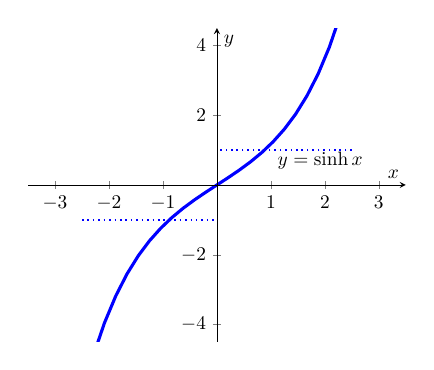
\begin{tikzpicture}[scale=0.7]
        \begin{axis}[
            xmin=-3.5, xmax=3.5,
            ymin=-4.5, ymax=4.5,
            axis lines=center,
            axis on top=true,
            domain=-2.5:2.5,
            ylabel=$y$,
            xlabel=$x$,]
            \addplot [mark=none,draw=blue,ultra thick] {sinh(\x)};
            \node [right, black] at (axis cs: 1,0.7) {$y = \sinh x$};
    
        %% Add the asymptotes
        \draw [blue, dotted, thick] (axis cs:-2.5,-1)-- (axis cs:0,-1);
        \draw [blue, dotted, thick] (axis cs:+2.5,+1)-- (axis cs:0,+1);
        \end{axis}
    \end{tikzpicture}
    \caption{Graph of F3} \label{fig:1.1}
    \end{figure}
Main characteristics of F3 is listed as below with proofs\cite{1}.

 \begin{itemize}
    \item F3 is one-to-one.
    \begin{equation}
        \frac{e^{m}-e^{-m}}{2} = \frac{e^{n}-e^{-n}}{2} \Leftrightarrow m = n
    \end{equation}
    
    \item F3 is onto.
    \begin{equation}
        \forall x \epsilon R, \exists y \epsilon R, \sinh x = y
    \end{equation}
        
    \item F3 is bijective function from \textbf{R} to \textbf{R}.
  \end{itemize}

\end{normalsize}

\begin{thebibliography}{1}
    
\bibitem{1}
mathcentre, Universities of Loughborough \\
\textit{http://www.mathcentre.ac.uk/resources/workbooks/mathcentre/hyperbolicfunctions}

\end{thebibliography}

\end{document}
